\chapter{System Hardware and Constraints}
\label{ch:hardware}

\section{Overview}
The experimental plant is a rotary (Furuta) inverted pendulum. A horizontal arm rotates about a vertical axis (base coordinate $\theta$). The pendulum is implemented as an \emph{L-shaped rod}: its horizontal segment forms a pivot shaft aligned with the arm (radial direction) and passes through three 688RS bearings mounted on the arm, while its vertical segment swings in the tangential--vertical plane (pendulum coordinate $\alpha$). The reference configuration is \emph{upright-only}, i.e., $\alpha=0$ corresponds to the pendulum held upright.

Figure~\ref{fig:rig_photo} shows the custom experimental rig used in this work.

\ThesisFigure{figures/rig_photo}{Photograph of the custom stepper-driven rotary (Furuta) inverted pendulum rig used in this work.}{fig:rig_photo}{0.95\linewidth}

This report is concerned with stabilization about the upright equilibrium and with servo-like base positioning while maintaining upright balance.

\section{Hardware build-up from scratch}
\label{sec:hardware_build}
To make the platform reproducible for students, the assembly was performed in the following dependency order:
\begin{enumerate}
  \item \textbf{Mechanical base and motor mount:} mount the stepper rigidly and verify shaft runout is acceptable before adding sensors.
  \item \textbf{Rotary arm and pendulum pivot:} install the rotary arm, then align the L-shaped pendulum shaft through the three 688RS bearings.
  \item \textbf{Base closed-loop retrofit:} convert the motor axis into a measured axis by adding the AS5600 housing and magnet assembly.
  \item \textbf{Driver and power wiring:} connect STEP/DIR/EN, \SI{24}{V} motor power, and common ground between motor supply, driver, and controller.
  \item \textbf{I\textsuperscript{2}C network and noise hardening:} connect both AS5600 sensors through PCA9548A channels and apply EMI-aware routing/shielding.
  \item \textbf{Calibration references:} define $\theta=0$ and $\alpha=0$ with multi-sample averaging before any closed-loop experiment.
\end{enumerate}
Sections~\ref{sec:mechanical_rig}--\ref{sec:sensing} detail each stage and the associated design constraints.

\section{Mechanical rig}
\label{sec:mechanical_rig}
The mechanical assembly consists of:
\begin{itemize}
  \item a rotary arm (yaw axis) driven by a stepper motor,
  \item an L-shaped pendulum assembly supported by a bearing-mounted pivot shaft (three 688RS bearings),
  \item mechanical hard-stops that bound the base rotation.
\end{itemize}

\subsection*{Actuation axis and coupling}
The arm is mounted coaxially to the stepper shaft (direct drive). The actuator is operated with a conversion of approximately $1600$ commanded steps per arm revolution:
\[
k_s \approx \frac{1600}{360} \approx \SI{4.444}{\step\per\degree},
\]
which is the conversion used throughout the firmware and analysis.

\subsection*{Converting the stepper into a closed-loop unit}
In open-loop operation, the commanded step count can diverge from the physical base angle due to missed steps, impulsive disturbances, or temporary stalls. To eliminate this ambiguity, the motor was retrofitted as a \emph{closed-loop single unit}: a 3D-printed AS5600 housing was fixed at the motor base, and the magnet mount was aligned coaxially with the rotating shaft so the base angle can be measured directly.

\begin{figure}[htbp]
  \centering
  \begin{subfigure}[t]{0.32\linewidth}
    \centering
    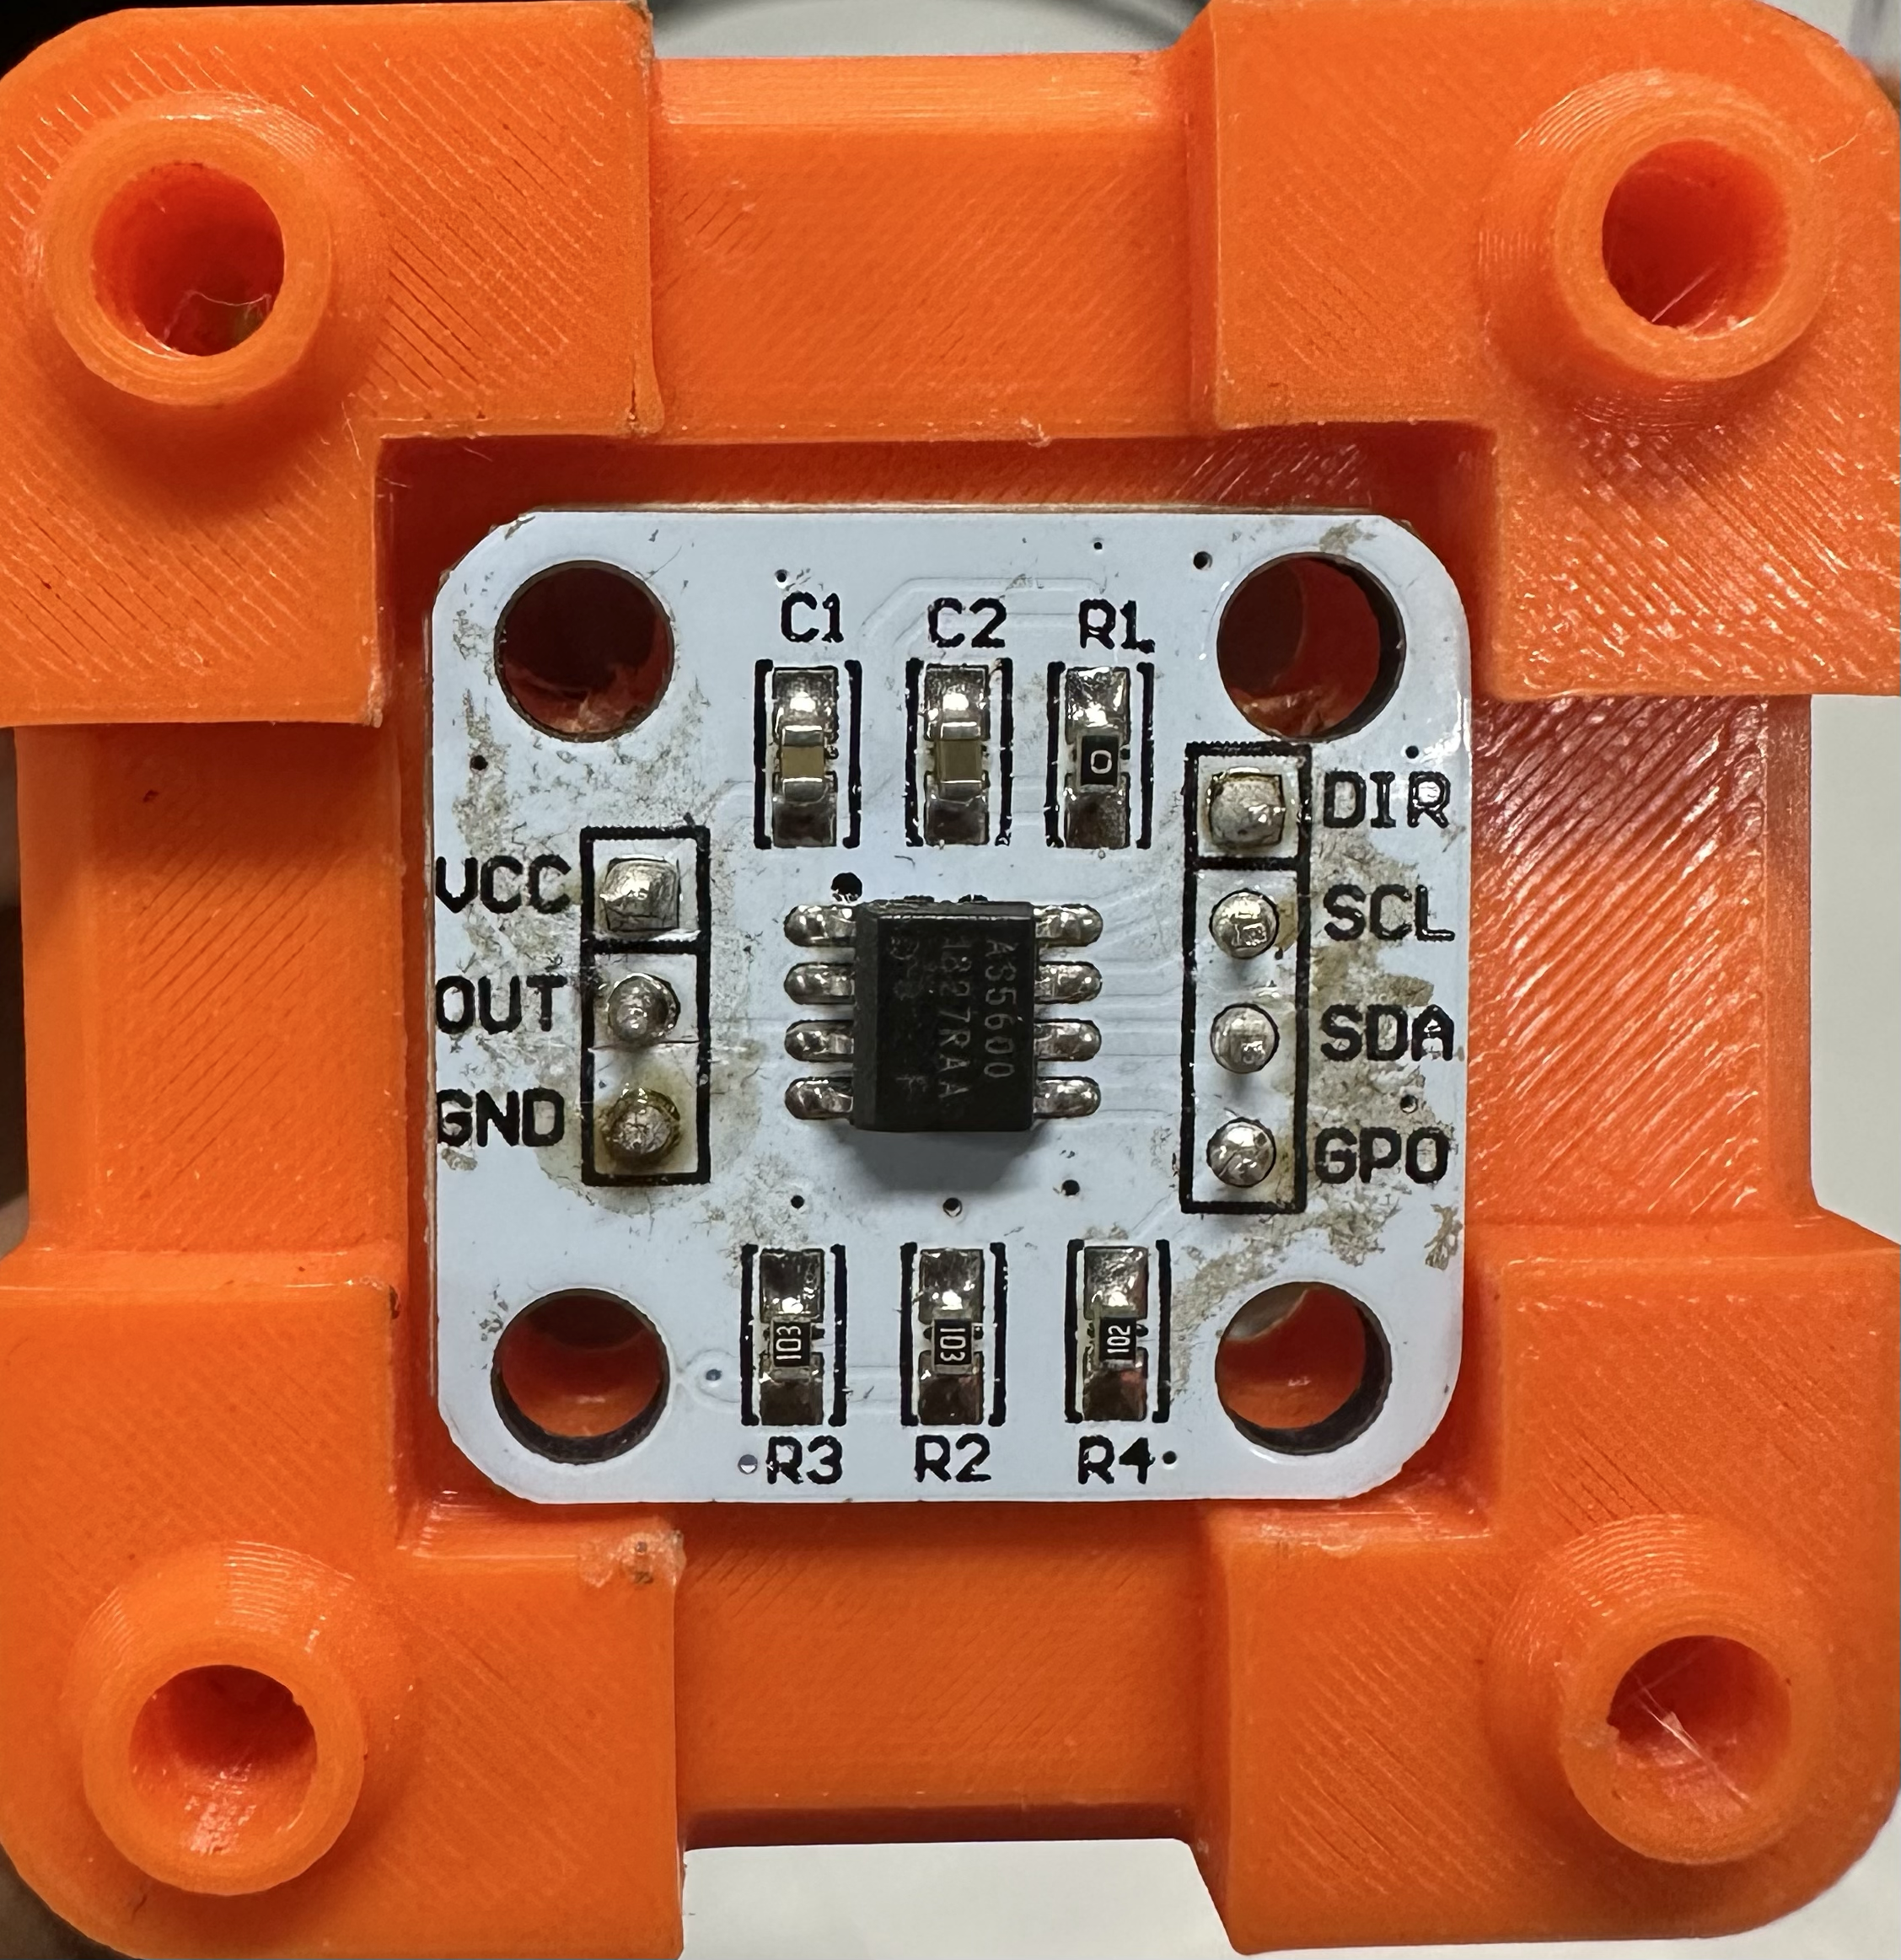
\includegraphics[width=\linewidth]{figures/sensor_housing_front.png}
    \caption{Front view of housing with sensor installed.}
    \label{fig:sensor_housing_front}
  \end{subfigure}\hfill
  \begin{subfigure}[t]{0.32\linewidth}
    \centering
    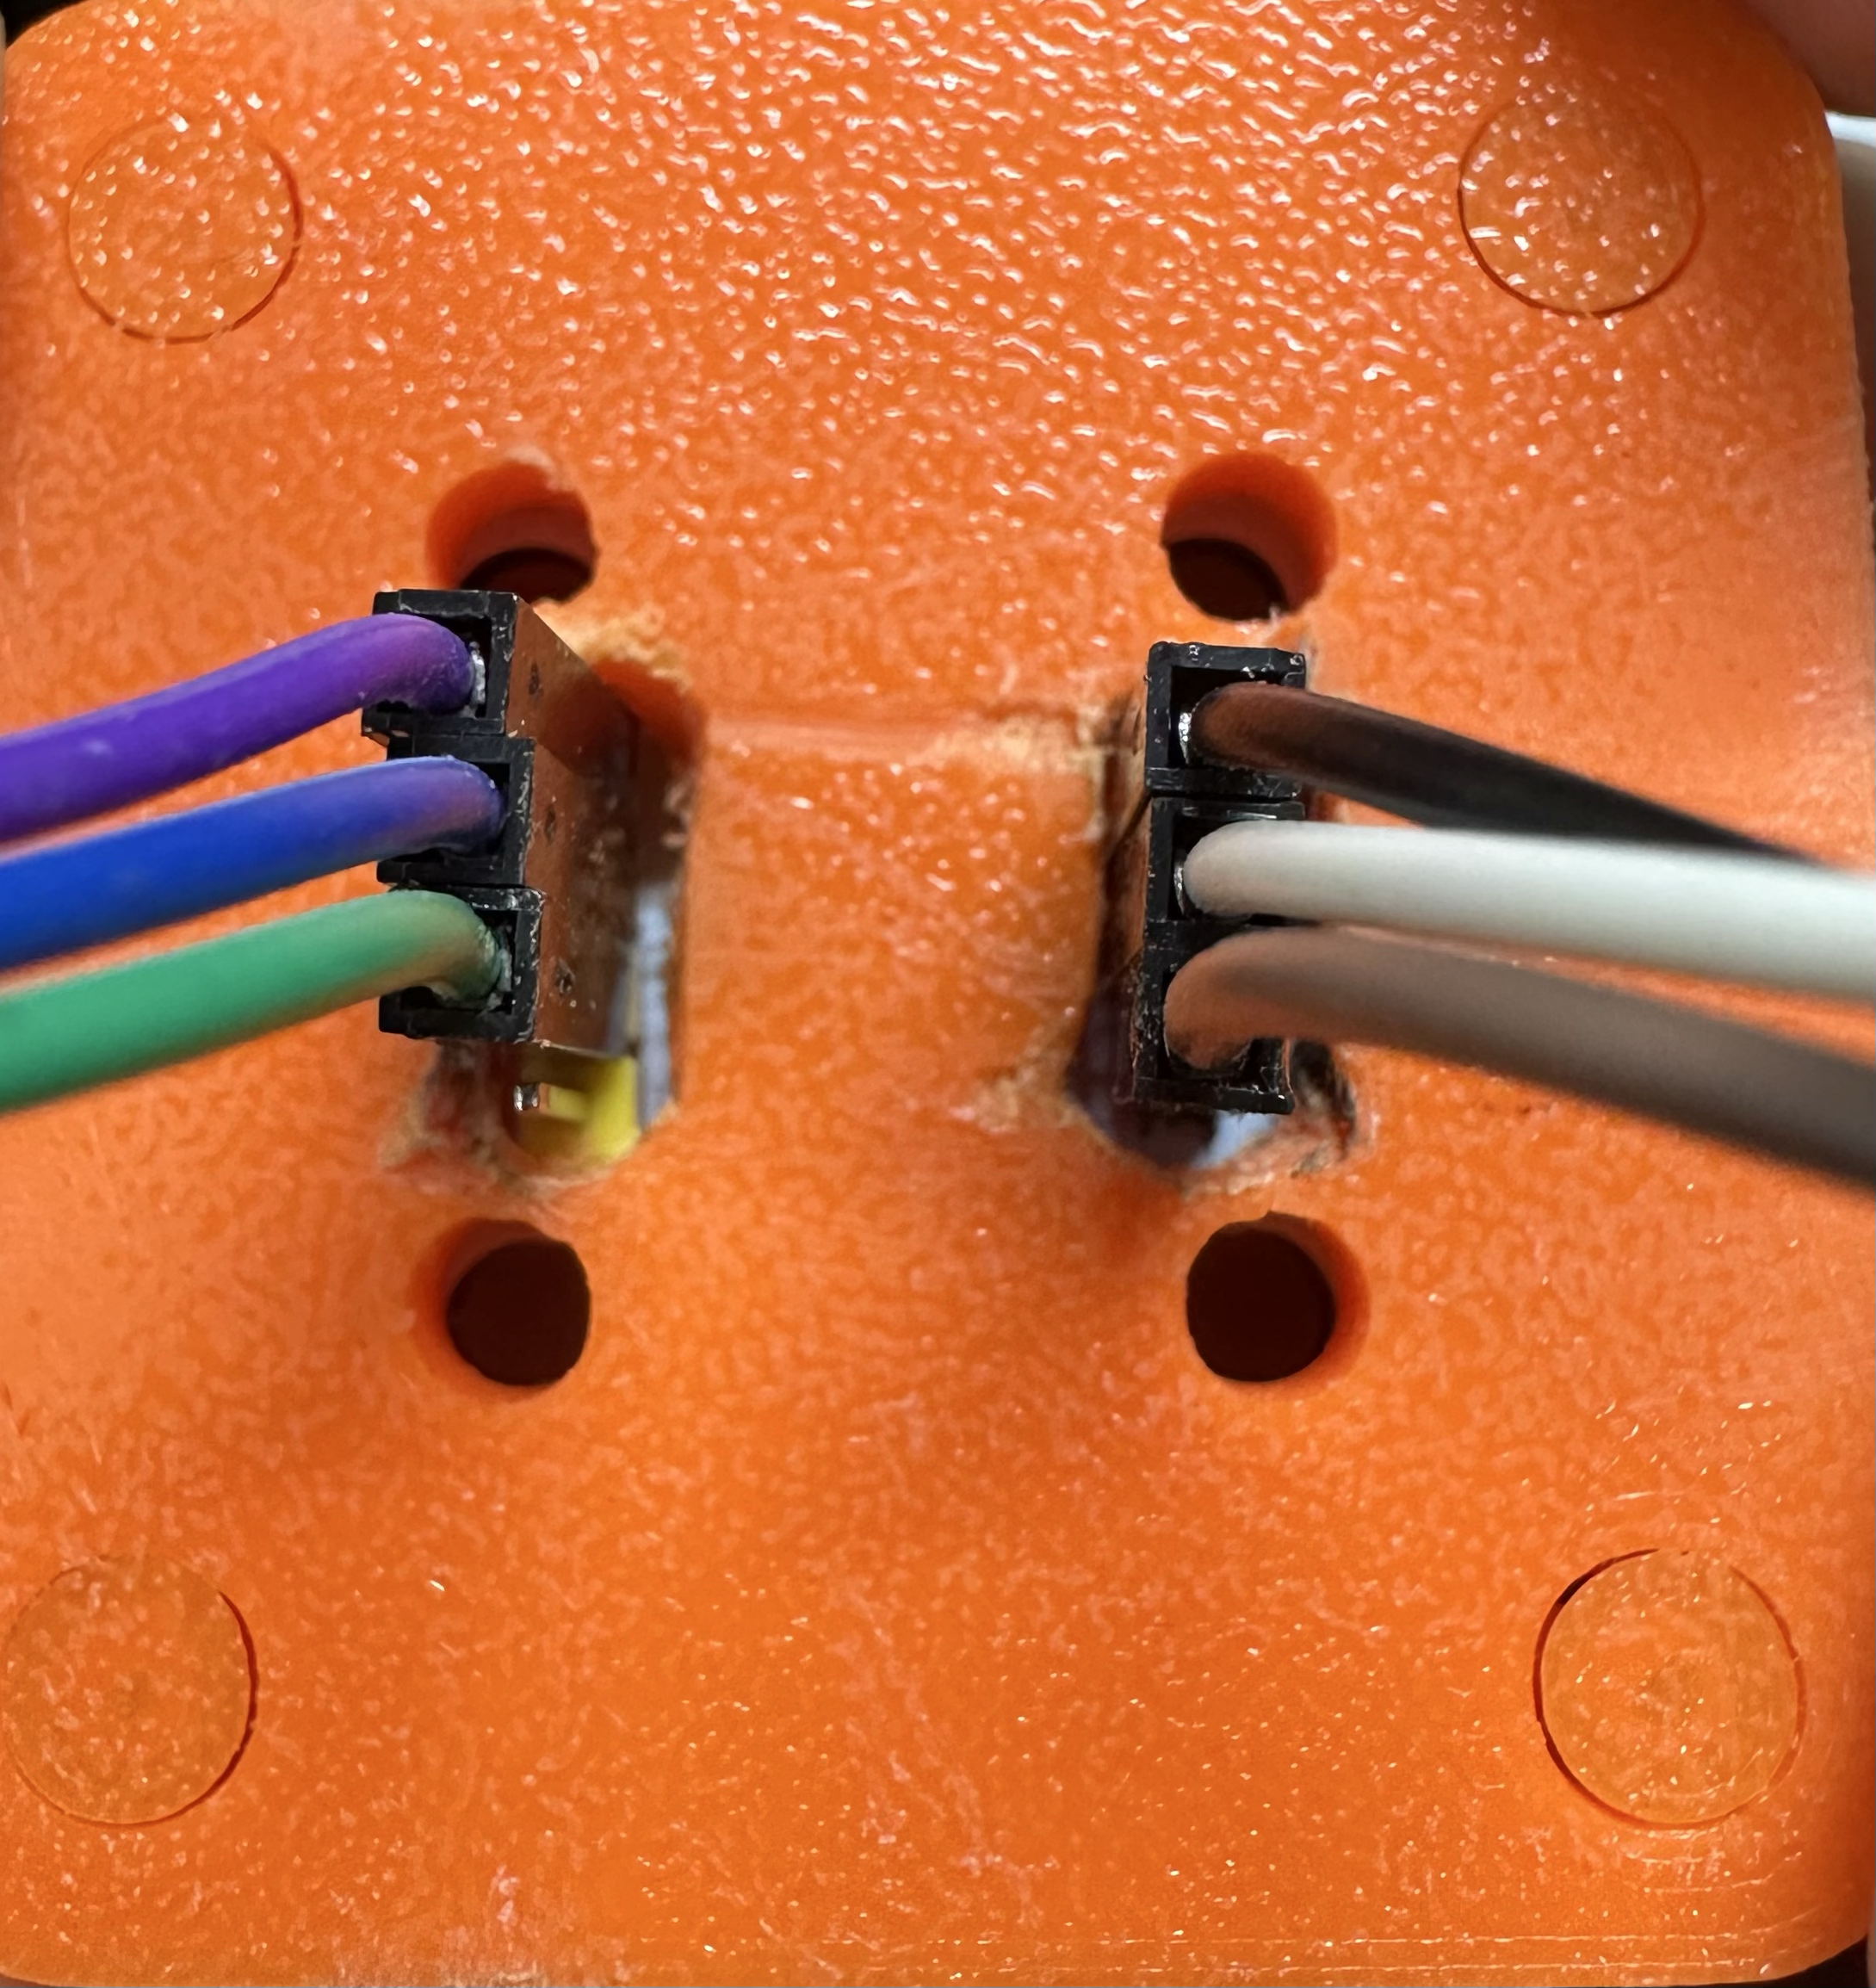
\includegraphics[width=\linewidth]{figures/sensor_housing_back.png}
    \caption{Back view showing mounting geometry.}
    \label{fig:sensor_housing_back}
  \end{subfigure}\hfill
  \begin{subfigure}[t]{0.32\linewidth}
    \centering
    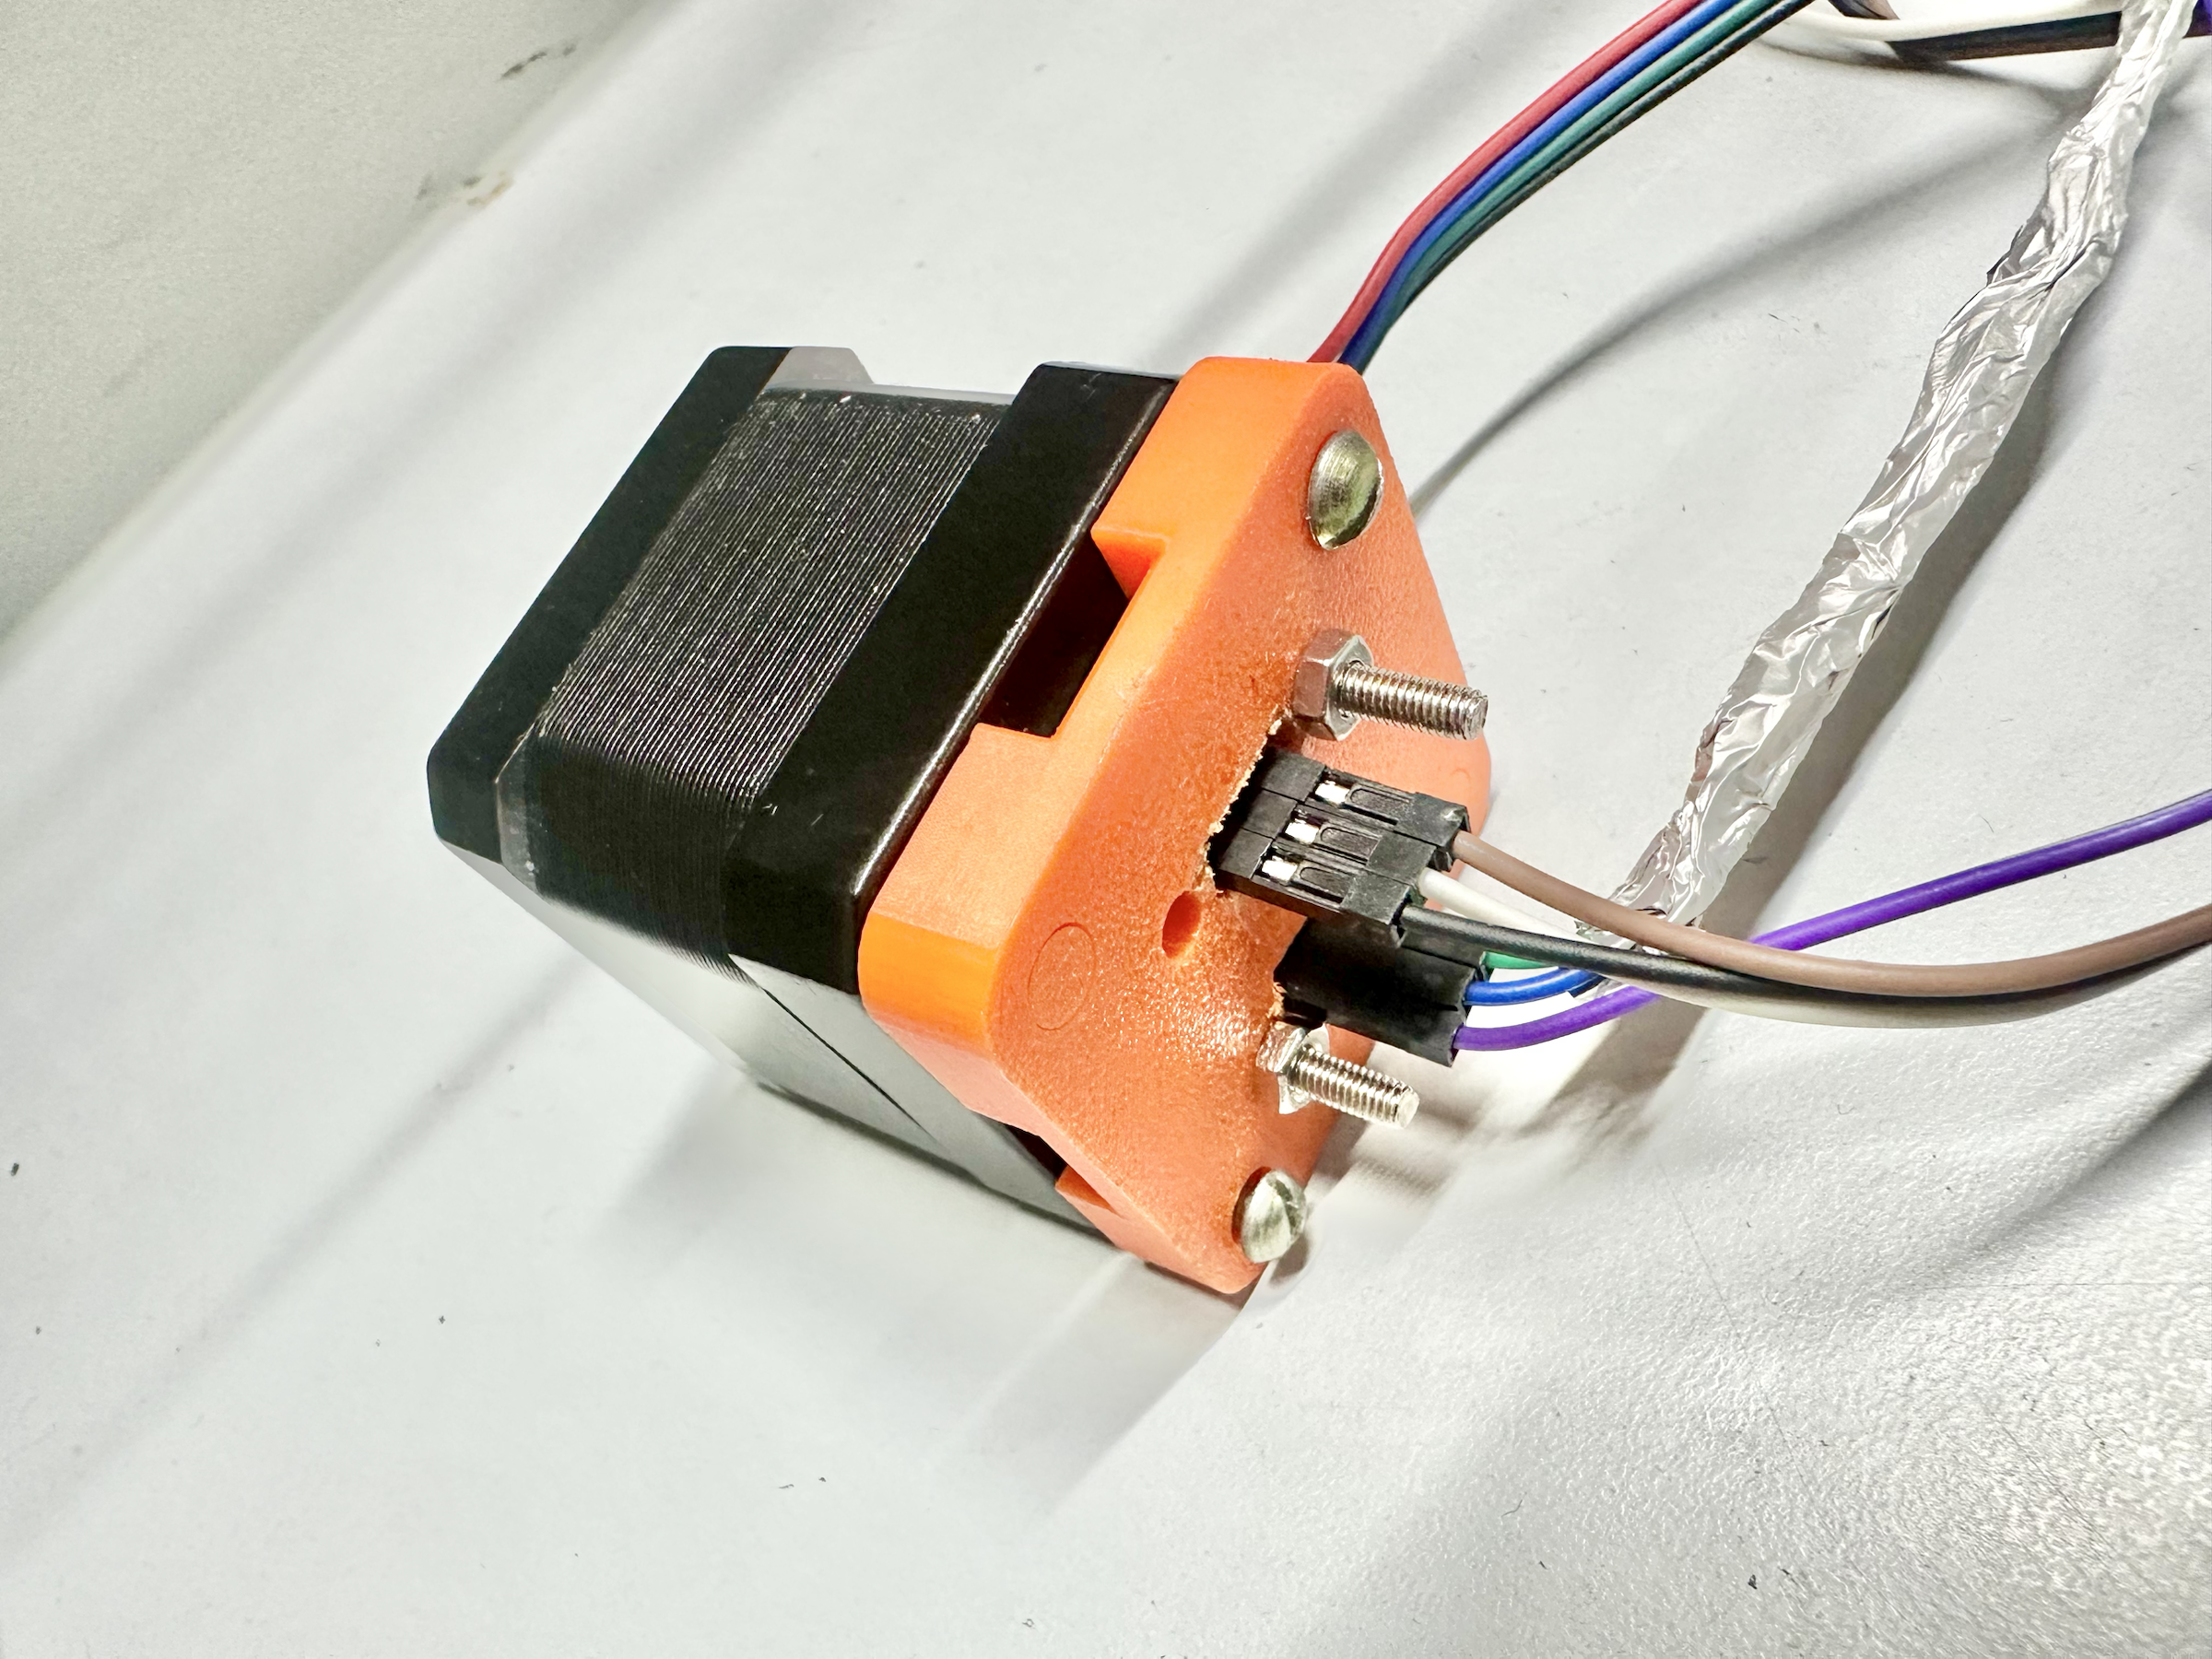
\includegraphics[width=\linewidth]{figures/sensor_housing_fixed_to_motor.png}
    \caption{Housing fixed to motor base (closed-loop unit).}
    \label{fig:sensor_housing_fixed_to_motor}
  \end{subfigure}
  \caption{3D-printed AS5600 housing used to convert the stepper into a closed-loop base actuator. For replication, the critical points are coaxial magnet alignment, rigid mounting, and consistent magnet-to-chip spacing. Small misalignment at this stage produces unstable angle data later in control experiments.}
  \label{fig:sensor_housing_closed_loop}
\end{figure}

\subsection*{Pendulum pivot (bearing-supported)}
The pendulum rotates about a bearing-supported pivot shaft that is aligned with the rotary arm. The shaft passes through three 688RS bearings, which reduce friction and minimize backlash in the pendulum degree of freedom (important because dissipative pivot dynamics couple directly into the required base acceleration for upright stabilization). The pivot assembly also carries the pendulum angle encoder magnet/fixture so the AS5600 measures $\alpha$ directly about this axis.

\subsection*{Key geometric parameters}
The main geometric and inertial parameters are derived and numerically identified in Chapter~\ref{ch:modelling}. For reference, the rig uses:
\begin{itemize}
  \item Arm length $L_r \approx \SI{0.19}{m}$
  \item Pendulum vertical length $L_v \approx \SI{0.12}{m}$ with a concentrated mass near the lower end
\end{itemize}

\section{Electronics and actuation}
\label{sec:electronics_actuation}
\subsection*{Controller and driver}
The base actuator is a stepper motor controlled by:
\begin{itemize}
  \item an Arduino Mega 2560 microcontroller (real-time control loop),
  \item a TMC2209 stepper driver (STEP/DIR/EN interface),
  \item a dedicated motor supply (\SI{24}{V}) separate from the Arduino \SI{5}{V} logic rail.
\end{itemize}
Motor power, driver, and microcontroller share a common ground. The driver supply is decoupled using a bulk electrolytic capacitor and a small ceramic capacitor close to the driver.

\subsection*{Driver and actuation settings}
\begin{table}[htbp]
  \centering
  \small
  \setlength{\tabcolsep}{6pt}
  \caption{Driver interface and actuation settings used in firmware.}
  \label{tab:driver_actuation_settings}
  \begin{tabularx}{\linewidth}{@{}l l X@{}}
    \toprule
    Setting & Value & Notes \\
    \midrule
    STEP/DIR/EN pins & D11 / D6 / D7 & Digital control outputs to the TMC2209 driver. \\
    I\textsuperscript{2}C bus clock & \SI{400}{kHz} & Multiplexer and AS5600 sensors share this bus speed. \\
    Base conversion & $1600$ steps/rev ($\SI{4.444}{\step\per\degree}$) & Conversion used in firmware for actuation and analysis. \\
    \bottomrule
  \end{tabularx}
\end{table}

\subsection*{Acceleration-input actuation model}
The driver is commanded in continuous-velocity mode (step rate in \si{\step\per\second}). To match this actuation pipeline, all controllers in this project are implemented in an \emph{acceleration-input form}: the controller computes a commanded base acceleration (in \si{\step\per\second\squared}), which is integrated in firmware to produce the commanded velocity:
\[
u \equiv \ddot{\theta} \ \longrightarrow\  \dot{\theta}_{\mathrm{cmd}} \ \longrightarrow\ \text{stepper speed command}.
\]
This is a central design choice: it makes the theoretical input used in modelling and control ($u=\ddot{\theta}$) coincide with the practical signal sent to the actuator (after integration to a velocity command).

\section{Sensing}
\label{sec:sensing}
\subsection*{Angle sensing}
Two AS5600 magnetic encoders measure absolute angles. Both devices share the same fixed I\textsuperscript{2}C address, so they are read through an I\textsuperscript{2}C multiplexer (PCA9548A, default address 0x70) at \SI{400}{kHz}:
\begin{itemize}
  \item Pendulum encoder (at the pendulum pivot axis)
  \item Base encoder (at the motor/base axis, see Figure~\ref{fig:sensor_housing_closed_loop})
\end{itemize}
Each AS5600 provides a \SI{12}{bit} absolute angle measurement over $[0,360^\circ)$ (nominal resolution $\approx \SI{0.0879}{\degree}$ per count).

\subsection*{Mechanical encoder mounting details}
Both pendulum and base sensors use:
\begin{itemize}
  \item a rigid printed housing to locate the AS5600 PCB relative to the rotating axis,
  \item a coaxial magnet mount attached to the rotating part,
  \item a controlled magnet-to-chip air-gap (typically \SIrange{2}{3}{mm}),
  \item mechanical features to reduce radial offset and wobble.
\end{itemize}
This reduces sensitivity to small misalignments that can otherwise cause jitter, dropouts, or inconsistent angle readings (all of which directly degrade derivative estimates and can destabilize the controller). The firmware additionally monitors AS5600 magnet-status diagnostics (detect/high/low) during certain fault conditions to help distinguish true actuator faults from sensor misalignment.

\subsection*{I\textsuperscript{2}C interference mitigation used in practice}
Because AS5600 links run close to a high-current stepper drive, the I\textsuperscript{2}C bus was treated as an EMI-sensitive interface. The baseline wiring rules used in this build were:
\begin{itemize}
  \item twist SDA and SCL together tightly and keep the run short,
  \item route I\textsuperscript{2}C wires away from motor phase wires and driver power loops,
  \item wrap the twisted pair with aluminium foil to create a simple shield,
  \item connect the foil shield to ground at the controller side only, leaving the sensor-side foil end floating.
\end{itemize}
This hardware practice reduced burst-like glitches caused by switching noise. Software-side protections (jump rejection and derivative-safe handling) are documented in Chapter~\ref{ch:measurement}, Section~\ref{sec:measurement_glitch_rejection}.

\subsection*{Calibration references}
Before each experimental trial, a short calibration routine averages multiple sensor samples (default: 25) to reduce single-sample noise and to define reference angles:
\begin{itemize}
  \item $\alpha=0$ reference: pendulum held upright
  \item $\theta=0$ reference: arm centered
\end{itemize}

\subsection*{Pin assignments (summary)}
For completeness, the essential microcontroller I/O used by the rig is:
\begin{table}[htbp]
  \centering
  \small
  \setlength{\tabcolsep}{6pt}
  \caption{Core I/O connections for the rig (Arduino Mega 2560).}
  \label{tab:pin_map}
  \begin{tabularx}{\linewidth}{@{}l p{0.28\linewidth} X@{}}
    \toprule
    Function & Arduino pins & Notes \\
    \midrule
    Stepper driver signals (STEP, DIR, EN) & D11 (STEP), D6 (DIR), D7 (EN) & digital outputs to the stepper driver \\
    I\textsuperscript{2}C bus (SDA/SCL) & D20 (SDA), D21 (SCL) & shared by PCA9548A and both AS5600 encoders \\
    I\textsuperscript{2}C multiplexer channels & ch0 (pendulum), ch1 (base) & selects which AS5600 encoder is visible on the bus \\
    \bottomrule
  \end{tabularx}
\end{table}

\section{Bill of materials}
\label{sec:bom}
Tables~\ref{tab:bom} and~\ref{tab:bom_passive} list the hardware required to reproduce the rig. Entries marked \texttt{TBD} are intentionally left open until the final procurement manifest is frozen.

\begin{table}[htbp]
  \centering
  \small
  \setlength{\tabcolsep}{4pt}
  \caption{Bill of materials (core subsystems).}
  \label{tab:bom}
  \begin{tabularx}{\linewidth}{@{}l c p{0.19\linewidth} p{0.18\linewidth} X@{}}
    \toprule
    Item & Qty & Spec/Model & Purpose & Notes/Source \\
    \midrule
    Microcontroller board & 1 & Arduino Mega 2560 & Real-time control and serial interface & Matches firmware pin map and loop implementation \\
    Stepper driver module & 1 & TMC2209 (STEP/DIR/EN) & Stepper current control and pulse interface & Base axis driver stage \\
    Stepper motor & 1 & 1.8\si{\degree}/step, model \texttt{TBD} & Base rotational actuation & Exact model/vendor \texttt{TBD} \\
    Motor power supply & 1 & \SI{24}{V} DC, current \texttt{TBD} & Dedicated motor rail & Repo indicates \SI{24}{V}; adapter model \texttt{TBD} \\
    Magnetic encoder modules & 2 & AS5600 & Absolute pendulum and base angle sensing & One on pendulum, one on base axis \\
    I\textsuperscript{2}C multiplexer & 1 & PCA9548A (0x70 default) & Allows two AS5600 devices on one I\textsuperscript{2}C bus & ch0 pendulum, ch1 base \\
    Encoder magnets & 2 & Diametric magnet, size \texttt{TBD} & Magnetic target for AS5600 & Maintain \SIrange{2}{3}{mm} air gap \\
    \bottomrule
  \end{tabularx}
\end{table}

\begin{table}[htbp]
  \centering
  \small
  \setlength{\tabcolsep}{4pt}
  \caption{Bill of materials (mechanical details and wiring passives).}
  \label{tab:bom_passive}
  \begin{tabularx}{\linewidth}{@{}l c p{0.19\linewidth} p{0.18\linewidth} X@{}}
    \toprule
    Item & Qty & Spec/Model & Purpose & Notes/Source \\
    \midrule
    Pendulum pivot bearings & 3 & 688RS & Low-friction pendulum pivot support & Bearing-supported L-pivot shaft \\
    Rotary arm assembly & 1 & Custom part, $L_r \approx \SI{0.19}{m}$ & Base arm geometry & Fabrication details \texttt{TBD} \\
    L-shaped pendulum assembly & 1 & Custom part, $L_v \approx \SI{0.12}{m}$ & Pendulum body and mass distribution & Includes pivot shaft and end mass \\
    Base encoder 3D-printed housing set & 1 set & Custom CAD print (\texttt{sensor\_housing\_*}) & Converts motor axis into measured closed-loop axis & See Figure~\ref{fig:sensor_housing_closed_loop} \\
    Pull-up resistors & 2 & \SI{5}{k\ohm}, tolerance \texttt{TBD} & SDA/SCL biasing & Final resistor package/tolerance \texttt{TBD} \\
    Driver bulk capacitor & 1 & \SI{100}{\micro\farad}, voltage \texttt{TBD} & VMOT rail smoothing & Place close to VMOT/GND pins \\
    Driver/sensor ceramic capacitors & \texttt{TBD} & \SI{0.1}{\micro\farad}, package \texttt{TBD} & High-frequency decoupling & One near VMOT and one per sensor supply \\
    Sensor local capacitors & 2 & \SI{1}{\micro\farad}, voltage \texttt{TBD} & Local AS5600 supply filtering & Final dielectric/package \texttt{TBD} \\
    Prototyping and wiring hardware & \texttt{TBD} & Breadboards, jumpers, foil shield, connectors & Electrical assembly and EMI mitigation & Counts depend on physical layout \\
    \bottomrule
  \end{tabularx}
\end{table}

\section{Host computer and data acquisition}
All experiments are run with a host computer connected over USB serial. A Python logger records:
\begin{itemize}
  \item a device-time CSV stream (angles, angular rates, command signals), and
  \item a text event stream (status lines and diagnostic messages).
\end{itemize}
These artifacts are later used to compute metrics and generate the figures/tables in the Results chapter.

\section{Safety limits and operating envelope}
The rig is operated under explicit safety limits for repeatability:
\begin{itemize}
  \item Base limit: $|\theta| > \SI{80}{\degree}$ triggers a safety disarm.
  \item Pendulum limit: $|\alpha| > \SI{30}{\degree}$ triggers a safety disarm.
  \item Upright-only validity window (nonlinear controllers): an additional hard abort is applied at $|\alpha|>\SI{25}{\degree}$ (and also at extreme $|\dot{\alpha}|$) to enforce ``no swing-up'' operation and to avoid numerically unsafe regions.
\end{itemize}

Limit checks are debounced across multiple control ticks to avoid false positives from single-sample sensor glitches. When a limit is confirmed, the motor output is disabled and the system returns to an idle state so the trial can be restarted safely.

\section{Replication notes and lessons learned}
\label{sec:replication_notes}
The most common bring-up failures in this project were: sensor noise spikes, magnet/housing misalignment, I\textsuperscript{2}C interference from motor wiring, and same-address encoder conflicts without multiplexing. The highest-leverage mitigation sequence was: establish rigid mechanical alignment first, verify magnet spacing and status bits, apply twisted-and-shielded I\textsuperscript{2}C wiring with one-end shield grounding, then enable software glitch rejection and calibration averaging. Following this order prevents repeated false debugging loops and makes educational replication significantly faster.
